% !TEX root = ../my-thesis.tex
%
\chapter{DESARROLLO TEÓRICO}
\label{sec:desarrollo teórico}

A lo largo de este capítulo, se desarrollara la teoría básica necesaria para la comprensión y desarrollo de este trabajo. Es por ello que será necesaria la explicación del funcionamiento de los Algoritmos Evolutivos, los Algoritmos Genéticos y de los parámetros que entran en juego dentro del mismo. De la misma manera, se realizará una introducción a la implementación de Redes Neuronales y más específicamente, a las Redes Neuronales Convolucionales, que serán el resultado final del trabajo.

\section{Algoritmos Evolutivos}

Los Algoritmos Evolutivos abarcan la resolución de problemas de optimización o búsquedas de soluciones dentro del ámbito de los algoritmos bio-inspirados \cite{10.5555/2432058}. Esto quiere decir que se basan en emplear analogías con sistemas naturales o sociales para el diseño de métodos heurísticos no deterministas.

Estos algoritmos además forman parte de una de las ramas de la inteligencia artificial. Básicamente su uso está bastante extendido en la resolución de problemas con espacios de búsquedas grandes y no lineales, donde otros métodos encuentran gran dificultad en encontrar alguna solución en un tiempo razonable.

En el uso de esto algoritmos se realizan a partir de una \textbf{población} de individuos, los cuales son posibles candidatos a solución de un problema. Esta se verá alterada tras una serie de procesos que nos llevará a encontrar mejores individuos o soluciones. Cada ciclo de transformación equivale a una \textbf{generación}. Después de cierto número de generaciones, se espera que los mejores individuos de esta población se localicen de forma bastante próxima a la solución esperada del problema.

Cada uno de los individuos de la población ha de ir codificado de tal manera que esta se vaya transmitiendo de generación en generación. Esta codificación también es conocida como \textbf{genotipo} y es la principal diferencia que existe entre los diferentes tipos de algoritmos evolutivos como veremos posteriormente. Este genotipo está formado por \textbf{genes} que es la pieza básica de información que codifica a nuestro individuo. Todos estos no pueden ser interpretados directamente, por lo que se necesita que a partir de esta codificación se forme la forma analizable del individuo.

A partir del genotipo, se han de formar los rasgos visibles del individuo, también conocido como \textbf{fenotipo}. Este es la representación directa de la información genética. Pueden darse casos en la que la codificación genética no siempre pueda formar una correspondencia directa en el fenotipo y que se deban dar unas condiciones determinadas, en las siguientes generaciones, para que cierta información genética se vea definitivamente representada en el individuo.

Como se puede ver, usando este tipo de algoritmos se combinan técnicas de búsqueda aleatoria, que viene dada por la transformación de la población, y búsqueda dirigida, dada por la selección de los individuos. Con esto se consigue abarcar un gran espacio de búsqueda, en relativamente poco tiempo, en comparación a otros algoritmos de optimización de problemas.

\subsection{Funcionamiento general}

Todos los algoritmos evolutivos tienen la similitud de que comparten un mismo esquema de funcionamiento. Estos vienen heredados de la teoría clásica de la evolución y emplean mecanismos evolutivos naturales como la reproducción, la mutación y la selección natural \cite{10.5555/2432058}.

\begin{figure}[h]
    \centering
    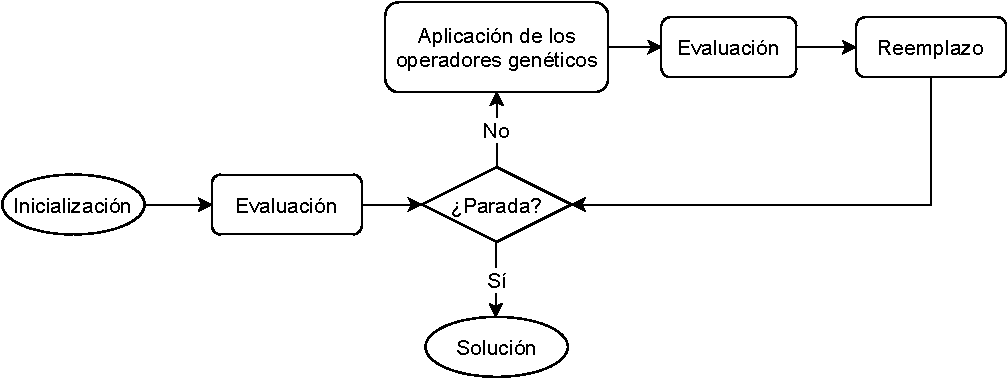
\includegraphics[width=\textwidth]{figuras/desarrollo teorico/Algoritmo_Evolutivo.pdf}
    \caption{Esquema de funcionamiento genérico de los Algoritmos Evolutivos}
    \label{fig:diagrama_alg_evolutivo}
\end{figure}

En la figura \ref{fig:diagrama_alg_evolutivo}, se describe el funcionamiento de un algoritmo evolutivo genérico. En él, se pueden ver las diferentes etapas por las que debe ir transitando cada uno de estos algoritmos.

En primer lugar, en la etapa de \textbf{inicialización} se crea una población del tamaño deseado, la cual esta compuesta por individuos que codifican diferentes soluciones muestreadas aleatoriamente dentro del espacio de búsqueda del problema. 

Como se veía anteriormente, cada individuo codifica una solución al problema propuesto y los operadores trabajan sobre esta codificación y no sobre las soluciones. Es por ello que es necesario posteriormente una etapa de \textbf{evaluación} donde se decodifica a este individuo y se obtiene la solución que representar para evaluar la calidad de este.

Si algunos de los individuos cumple los criterios dados para la solución del problema, se termina el algoritmo y se devuelven las mejores soluciones. De no ser así, se comienza un proceso iterativo en el cual se aplican diferentes \textbf{Operadores Genéticos} basados en los mecanismos evolutivos naturales para obtener nuevas soluciones que reemplacen a las antiguas. A cada iteración se la denomina \textbf{generación}.

Posteriormente, se debe volver a \textbf{evaluar} a todas las nuevas soluciones tal y como realizábamos anteriormente. Esto simula el desempeño de las tareas más importantes para la supervivencia de un individuo.

Una vez conocido el desempeño de las diferentes soluciones, se debe proceder a generar la población de la siguiente generación. Esto se realiza mediante la operación de \textbf{reemplazo}. Esto es debido a que se toma una población constante que simula un medio con recursos finitos, en los que los individuos deben competir entre ellos por la supervivencia dentro del grupo. En este paso es importante mantener la diversidad genética dentro de la población, por lo que se proponen técnicas donde todos los individuos tienen cierta probabilidad de sobrevivir asociado a su desempeño.

Tras esto, se debe verificar la \textbf{condición de parada} nuevamente, para determinar si se debe continuar con la ejecución del algoritmo o se debe proceder a salir del proceso iterativo. Se espera que con cada iteración el desempeño medio de la población vaya incrementándose hasta su convergencia en un óptimo o una solución definitiva.


\subsection{Clasificación de Algoritmos Evolutivos}

Como ya se veía anteriormente, existen numerosas técnicas de replicar el comportamiento evolutivo de los seres vivos en diferentes tipos de algoritmos. Esta división viene dada básicamente por la forma que toma el genotipo o codificación de los diferentes individuos de la población.

Esto alterará de forma inmediata la forma en la que los diferentes genotipos realizan las diferentes operaciones de mutación y cruce, por lo que se tienen que definir nuevos operadores para cada uno de estos tipos de algoritmos evolutivos.

Existen tres aproximaciones principales para estos mecanismos: los algoritmos genéticos, las estrategias evolutivas y la programación genética.

Los \textbf{Algoritmos Genéticos} \cite{Holland1984} emplean una codificación binaria, por lo que cada gen del genotipo esta formado por un valor ``0'' o ``1'' según corresponda. En la figura \ref{fig:ej_AG} podemos ver un ejemplo de esta representación.

Por otro lado, las \textbf{Estrategias Evolutivas} \cite{Beyer2002} se diferencian de las anteriores que la codificación se basa en el uso de número naturales que pueden ser representados de forma continua o discreta, según el problema. En la figura \ref{fig:ej_EE} podemos ver un ejemplo de esta representación.

Por último, en la \textbf{Programación Genética} \cite{koza1992genetic} la representación de los individuos es bastante diferente a los anteriores, y es que se emplean estructuras de arboles. En ella cada nodo del árbol expresa una función como operador y cada terminal del nodo, por el contrario, contiene un operando, por lo que se pueden generar expresiones de manera bastante sencilla. En la figura \ref{fig:ej_PG} podemos ver un ejemplo de esta representación.

\begin{figure}[h!]
\centering
    \begin{subfigure}{0.51\textwidth}
        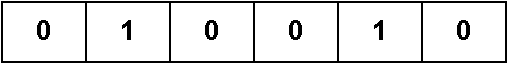
\includegraphics[width=\textwidth]{figuras/desarrollo teorico/Algoritmo_Evolutivo-ej_AE.pdf} 
        \caption{Algoritmo Genético}
        \label{fig:ej_AG}
    \end{subfigure}
    \begin{subfigure}{0.51\textwidth}
        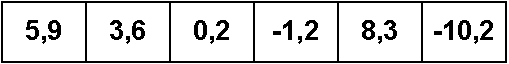
\includegraphics[width=\textwidth]{figuras/desarrollo teorico/Algoritmo_Evolutivo-ej_EE.pdf}
        \caption{Estrategias Evolutivas}
        \label{fig:ej_EE}
    \end{subfigure}
    \begin{subfigure}{0.65\textwidth}
        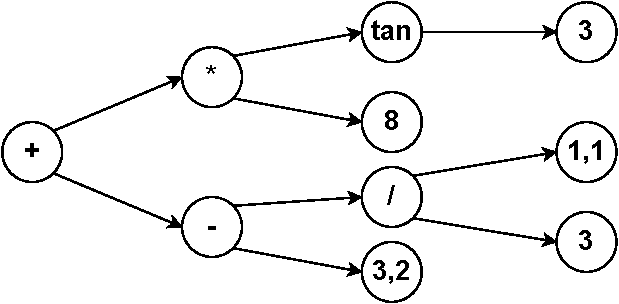
\includegraphics[width=\textwidth]{figuras/desarrollo teorico/Algoritmo_Evolutivo-ej_PG.pdf}
        \caption{Programación genética}
        \label{fig:ej_PG}
    \end{subfigure}
\caption{Ejemplos de representación de los diferentes tipos de Algoritmos Evolutivos}
\label{fig:ej_AE}
\end{figure}

\section{Algoritmos genéticos}

Los Algoritmos Genéticos vienen establecidos por Holland desde el año 1975 \cite{Holland1984} y posteriormente descritos de forma precisa en numerosos libros y artículos \cite{GoldbergDavidE.DavidEdward1989Gais}. En estos se demuestra como se trata de una técnica robusta y como puede solucionar con bastante éxito una amplia variedad de problemas a resolver de diferentes áreas.

Cabe destacar también, que este tipo de algoritmos cuentan con bastantes debilidades al no garantizar, por ejemplo, la localización de una solución óptima al problema a resolver. A pesar de esto, se demuestra empíricamente que el nivel de calidad de las soluciones es más que aceptable, y sobretodo, realizándolo en un tiempo competitivo con respecto a otras técnicas más especializadas de resolución de ciertos problemas.

Como ya se ha visto anteriormente, los Algoritmos Genéticos vienen dados por una codificación binaria del genotipo, lo que establece una forma de operar determinada, que lo diferencia del resto de Algoritmos Evolutivos.

En algunos problemas, puede que se tenga la necesidad que pequeños cambios en el genotipo resulten en pequeños cambios en el fenotipo, por lo que se puede acudir a codificaciones como la de Gray.

En las próximas páginas, se irá mostrando el funcionamiento y los parámetros que forman parte de este tipo de algoritmos y que son necesarios conocer, para la resolución posterior de forma adecuada de un problema determinado.

\subsection{Funcionamiento general}

El funcionamiento general de los Algoritmos Genéticos, se basan en lo ya visto en el funcionamiento general de los Algoritmos Evolutivos.

\begin{figure}[h]
    \centering
    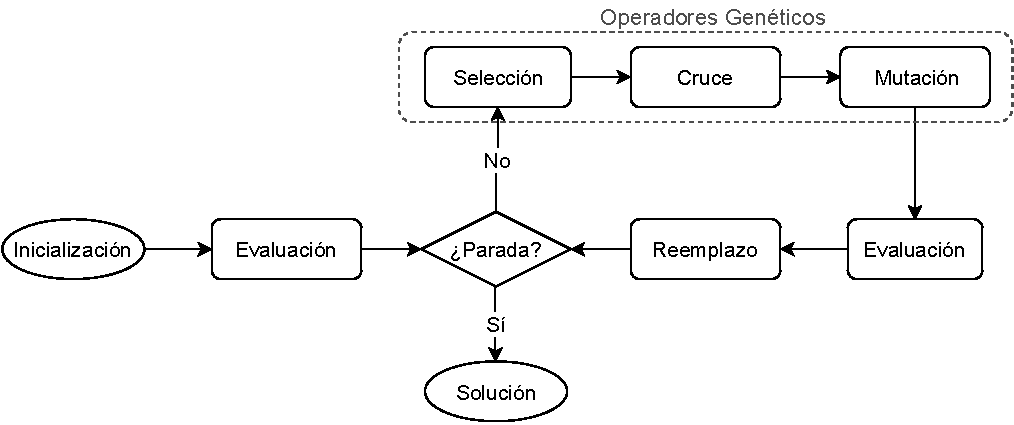
\includegraphics[width=\textwidth]{figuras/desarrollo teorico/Esquema_algoritmo_genetico.pdf}
    \caption{Esquema de funcionamiento de Algoritmos Genético Simple}
    \label{fig:diagrama_alg_genetico}
\end{figure}

En la figura \ref{fig:diagrama_alg_genetico}, se puede observar como se muestran los tres operadores genéticos que serán necesarios para la generación de nuevos individuos que serán candidatos a reemplazar generacionalmente a la anterior población.

Estos tres operadores son la \textbf{selección}, donde se deben seleccionar a los padres para la reproducción, el \textbf{cruce} donde con cierta probabilidad los padres generaran a los hijos y finalmente la \textbf{mutación}, donde nuevamente con cierta probabilidad aplicará una alteración en el genotipo en los hijos.

\subsection{Selección}

La selección de los padres es una operación que ha de realizarse de forma aleatoria, implementado diferentes técnicas para favorecer que los mejores individuos de una población a ser elegidos para posteriormente realizar el cruce con otro padre seleccionado.

Es importante en este paso garantizar que los mejores individuos de la población tengan mayor probabilidad de reproducirse frente a otros menos buenos. Aún así, hay que tener la cautela de dar oportunidad de selección a individuos menos buenos, ya que estos pueden portar en su genotipo partes útiles para el proceso de reproducción.

Existen diferentes estrategias de selección que pueden ser seguidas en función del problema que se esté tratando de resolver. Entre ellas encontramos la selección por torneo, el ranking lineal, la selección aleatoria, el emparejamiento variado inverso y la selección por ruleta.

\begin{itemize}
    \item La \textbf{Selección por Torneo} (TS) es una de las estrategias más empleadas. En ella, la selección se basa en la generación de diferentes ``torneos'' o grupos de individuos escogidos al azar de la población. En estos se selecciona al mejor individuo entre ellos. La manera en el que se seleccionan los individuos se ajusta en función a la cantidad de participantes en el torneo. A mayor cantidad de individuos en un torneo, menor probabilidad de seleccionar a individuos menos buenos.
    
    \item En el \textbf{Ranking Lineal} (LR), la población se ordena en función de lo bueno que es el cada uno de los individuos. Esto se asocia a una probabilidad de selección de cada uno de los individuos en función de la posición que tomen cada uno de ellos. De esta manera se le da mayor probabilidad de selección a los mejores individuos.
    
    \item En la \textbf{Selección Aleatoria} (RS), como su nombre indica, se seleccionan a los individuos de forma azarosa. Esto quiere decir que no se mira que tan bueno es el individuo para seleccionarlo como padre.
    
    \item El \textbf{Emparejamiento Variado Inverso} (NAM), es un método que trata de buscar una selección de padres con carga genética diferente y evitar que dos individuos muy parecidos se reproduzcan después. Esto lo realiza mediante la selección de un padre aleatoria. Posteriormente se seleccionan un número N de padres y se escoge entre ellos el cual contenga más diferencias en el genotipo con el primer padre seleccionado.
    
    \item La \textbf{Selección por Ruleta} es el método más empleado para la selección de padres dentro de los Algoritmos Genéticos. En este se asigna una probabilidad de selección proporcional a la calidad del individuo y se selecciona a uno aleatoriamente.
    
\end{itemize}

La selección de una u otra estrategia de selección dependerá de las necesidades del problema a optimizar.


\subsection{Cruce}

El cruce los padres se asocia a la fase reproductiva de los individuos de la población en la cual se han de mezclar la información genética de los individuos seleccionados. Esto dará como lugar la creación de nuevos individuos que representarán los candidatos a individuos de la siguiente generación.

El cruce se realiza como forma de exploración guiada cerca de las soluciones conocidas, tratando de buscar los mejores genes en una zona local.

Para la realización de este cruce, se asocia a él una probabilidad por la cual establece cuando una pareja de padres generará o no descendencia. Normalmente se suelen seleccionar valores altos de probabilidad, entre el 0,6 y el 0,9 aproximadamente. Esto dependerá del problema que se esté tratando a resolver.

Además se piden más aspectos a tener en cuenta para la realización de este cruce, y es que los hijos deben heredar algunas de las características de cada uno de los padres. También, el resultado debe ser un genotipo válido y que conserve la forma definida dentro del problema. Destacar además que los genotipos creados deben ser capaces de generar, de la manera que se ha definido, fenotipos válidos para la resolución del problema.

Existen diferentes estrategias a seguir para la realización de este cruce, entre las que encontramos: el cruce en un punto, el cruce en N puntos y el cruce uniforme.

\begin{itemize}
    \item El \textbf{Cruce en un punto} (\textit{1-point Crossover}) se basa en la selección de un punto de cruce aleatorio dentro del genotipo de ambos padres. Los padres se dividen a partir de ese punto y se crean hijos intercambiando partes de los genotipos. Es por ello que el resultado de aplicar este son dos hijos con información genética de ambos padres.
    
    En la Figura \ref{fig:cruce_1_punto}, se puede ver un ejemplo de esta operación.\\
    
    \begin{figure}[h]
         \centering
         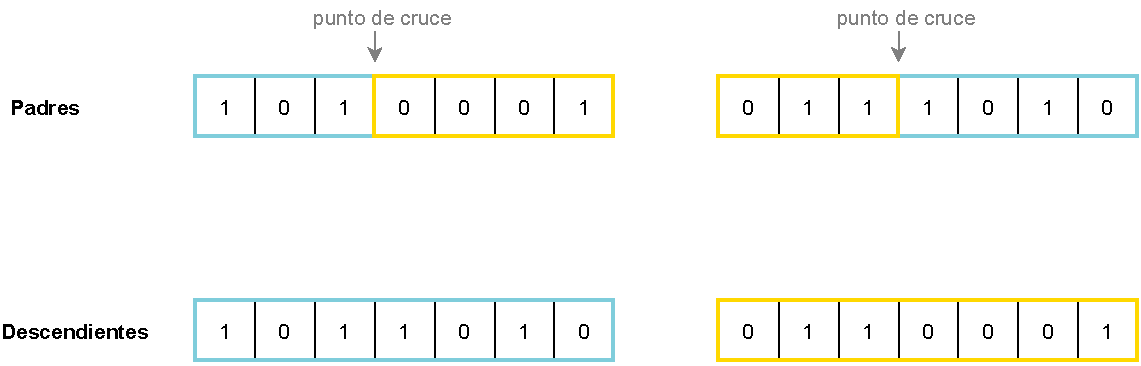
\includegraphics[width=1.1\textwidth]{figuras/desarrollo teorico/cruce_1_punto.pdf}
         \caption{Ejemplo de cruce en un punto}
         \label{fig:cruce_1_punto}
    \end{figure}
    
    Hay que tener diferentes cosas en cuenta, como que depende del orden en el que van apareciendo los genes y por lo tanto guarda un sesgo posicional, que depende del problema a resolver, este puede ser beneficioso o perjudicial.
    
    \item El \textbf{Cruce en N puntos} (\textit{N-point Crossover}) es una generalización del cruce en un punto anteriormente comentado. En este en vez de seleccionar tan solo un punto de corte, se seleccionan N puntos. Esto ayuda a que se fragmente de mayor medida la información genética de ambos padres.
    
    En la Figura \ref{fig:cruce_N_puntos}, se puede ver un ejemplo de la aplicación de esta operación.\\
    
    \begin{figure}[h]
         \centering
         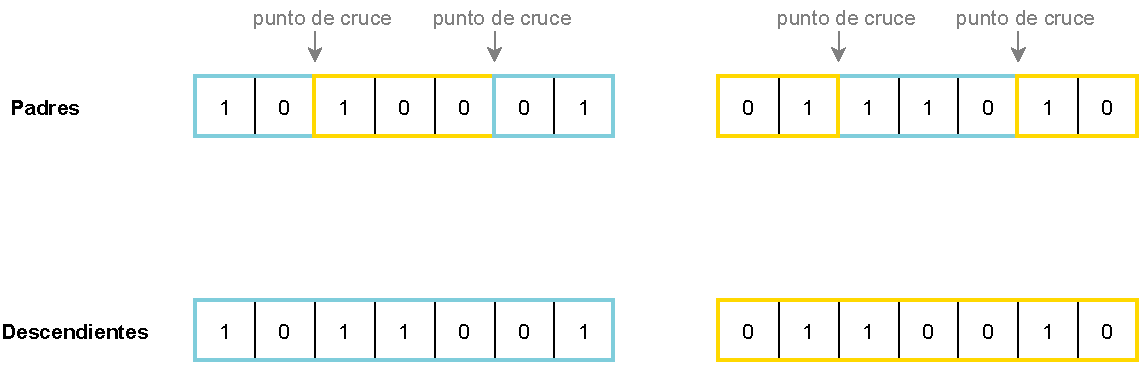
\includegraphics[width=1.1\textwidth]{figuras/desarrollo teorico/cruce_N_puntos.pdf}
         \caption{Ejemplo de cruce en dos puntos}
         \label{fig:cruce_N_puntos}
    \end{figure}
    
    \item Por último encontramos el \textbf{Cruce Uniforme} (\textit{Uniform Crossover}). En este la mezcla de información genética se realiza de forma aleatoria, en la cual se selecciona con cierta probabilidad por la que un determinado gen debe intercambiarse a lo largo del genotipo de ambos padres. En la Figura \ref{fig:cruce_uniforme}, se puede ver un ejemplo de la aplicación de esta operación.\\
    
    \begin{figure}[h]
         \centering
         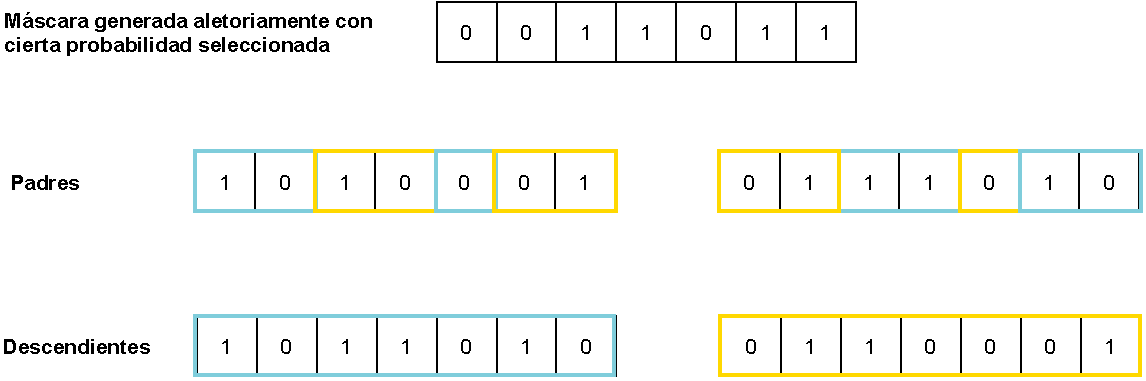
\includegraphics[width=1.1\textwidth]{figuras/desarrollo teorico/cruce_uniforme.pdf}
         \caption{Ejemplo de cruce uniforme}
         \label{fig:cruce_uniforme}
    \end{figure}

    En este tipo de cruce, la herencia del gen es independiente de su posición dentro del genotipo, por lo que se elimina el sesgo posicional que encontrábamos en las anteriores estrategias.

\end{itemize}


\subsection{Mutación}

La mutación es una operación que se realiza de forma individual a cada uno de los individuos de la población. Esto significa que se modifica el valor al azar de alguno de los genes del cromosoma de un individuo seleccionado de forma aleatoria dentro de nuestra población.

Esta operación es importante dentro del algoritmo, porque permite la exploración extensiva del espacio de búsqueda del problema, que solo con la operación de cruce no sería posible realizar. Esto es de vital importancia para asegurar la correcta convergencia del Algoritmo Genético.

La mutación es una operación bastante sencilla de implementar, ya que tan solo hay que definir una probabilidad por la que un individuo va a ser seleccionado para que mute. Esta probabilidad normalmente debe ser baja, para evitar convertir el algoritmo en un método de exploración aleatoria.

Posteriormente, tras tener el individuo seleccionado, se proporciona una nueva probabilidad a cada gen de su cromosoma para ser mutado, y en caso positivo, se cambia el valor de ese gen. El valor de este depende del problema a resolver.

En la Figura \ref{fig:mutacion}, se puede ver un ejemplo de esta operación.\\

\begin{figure}[h]
         \centering
         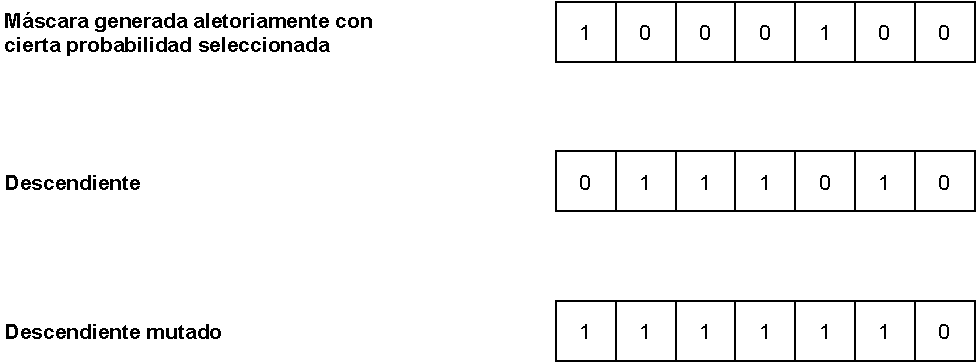
\includegraphics[width=\textwidth]{figuras/desarrollo teorico/mutacion.pdf}
         \caption{Ejemplo de operación de mutación}
         \label{fig:mutacion}
    \end{figure}

\subsection{Evaluación}

La evaluación es una de las fases más críticas dentro del algoritmos, ya que su definición de manera no adecuada, puede llevar a nuestro problema de optimización a no conseguir los resultados esperados.

En esta fase, se debe a partir del fenotipo del individuo, obtener un valor real el cual refleja el nivel de adaptación o desempeño que ha tenido este como solución a nuestro problema.

Esta evaluación se realiza normalmente a partir de una función objetivo o función \textit{fitness}. Esta vendrá dado por una expresión o por una métrica obtenida a partir del fenotipo del individuo en cuestión.

Esta nos interesa que cumpla cierta regularidad, por lo que dos individuos que se encuentren cercanos dentro del espacio de búsqueda, serán parecidos sus valores de \textit{fitness}.

Suele ser normal además, el establecer una penalización dentro de la propia función \textit{fitness}, debido a que puede haber zonas del espacio de búsqueda que no son deseadas o válidas, por lo que esto debe quedar reflejado en el desempeño de la solución encontrada.

\subsection{Reemplazo}

El reemplazo es el proceso por el cual se sustituyen a todos o a ciertos padres de la anterior población, por el resultado de las operaciones genéticas, a los que denominamos hijos.

Este proceso modela la limitación de recursos suficientes para todos los individuos de la población, por lo que se debe intentar mantener una población determinada o máxima.

Existen diferentes formas de plantear este proceso. Algunos vienen dados en función del número de hijos que sustituyen a cierto numero de padres. Estos modelos son: los Modelos Generacionales y Estacionarios.

\begin{itemize}
    \item El \textbf{Modelo Generacional} se caracteriza por que en cada generación, se crea un población totalmente nueva que sustituye íntegramente a la población anterior.
    \item El \textbf{Modelo Estacionario} donde los nuevos individuos reemplazan a uno o varios de los padres, pero no a todos. Es un modelo en el cual se trata de que los mejores individuos prosigan tras varias generaciones.
\end{itemize} 

Dentro de los Modelos Estacionarios encontramos diferentes estrategias para el reemplazo como son: Reemplazar al peor de la población, Torneo Restringido, Peor entre semejantes, y Algoritmo de Crowding Determinístico.

\subsection{Elitismo}

En ocasiones, se requiere la conservación de los mejores individuos a lo largo de las diferentes generaciones para que siga dando de su buena información genética a los nuevos individuos de la población.

Es por ello, que las medidas de selección en función de lo bueno que es el individuo pueden no asegurar siempre la supervivencia de estos dentro de la población, por lo que a veces es necesario asegurar su no desaparición de la población.

Para este problema se crea la estrategia denominada \textbf{Elitismo}, por la cual se protegen a los mejores individuos de una población ante los mecanismos de selección, cruce y mutación, conservándolos intactos en la siguiente generación.

Este mecanismo bajo ciertas condiciones generales, garantiza la convergencia en un óptimo global y además en la práctica ayuda a una mejora de la velocidad de obtención de buenos resultados.



\section{Redes Neuronales Artificiales}

Las Redes Neuronales Artificiales se engloban dentro de las técnicas de aprendizaje automático o aprendizaje máquina (\textit{Machine Learning}) como algoritmos bio-inspirados \cite{10.5555/523781}, al igual que se veía con los Algoritmos Evolutivos.

Estas técnicas, sin embargo, tratan de imitar el funcionamiento biológico simplificado de las neuronas que componen el cerebro. Al igual que el cerebro, la interconexión de gran cantidad de estas neuronas se tratan de emplear para la resolución de problemas como la memorización o la clasificación, entre otras.

Este Aprendizaje Automático donde se engloba este algoritmo, tiene como fin el desarrollo de sistemas que de forma autónoma y en base a la experiencia, sean capaces de cambiar su comportamiento, consiguiendo la capacidad de aprender a partir de unos datos dados. 

El aprendizaje automático se divide en dos tipos: el Aprendizaje Supervisado y el Aprendizaje No Supervisado. Las Redes Neuronales Artificiales forman parte del primer grupo, ya que los datos de entrada que recibe, van etiquetadas, de manera que es capaz de asociar el dato con la etiqueta correspondiente.

\subsection{Estructura y funcionamiento}

Para realizar la explicación del funcionamiento de las redes neuronales artificiales, se comenzará describiendo la red neuronal más simple existente. Esta está formada por una neurona y una única entrada \cite{10.5555/523781}. En la figura \ref{fig:neurona_simple}, se puede ver el esquema de esta red representada.

\begin{figure}[h]
    \centering
    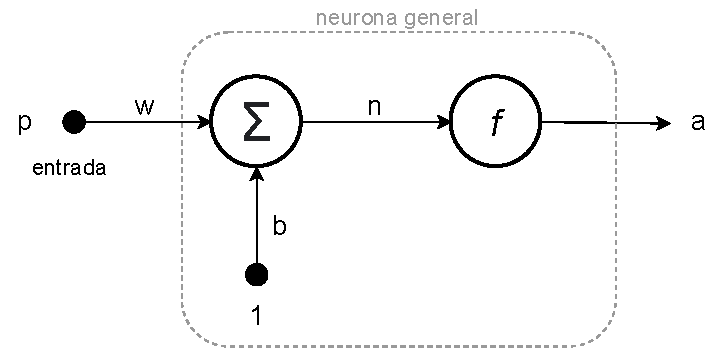
\includegraphics[width=0.7\textwidth]{figuras/desarrollo teorico/neurona.pdf}
    \caption{Esquema simple de una neurona artificial de una entrada y una salida}
    \label{fig:neurona_simple}
\end{figure}


El funcionamiento de esta es muy simple. En la entrada, se recibe un escala $p_1$ que es multiplicado por un peso $w_1$. Esto entra dentro de un sumatorio donde se entrarán además el resto de entradas en caso de tenerlas. Además, al sumatorio entra una señal de \textit{bias} representado por la letra $b$ en nuestro esquema. Por simplificación, esta señal se modela como una entrada siempre a 1 multiplicada por un valor $w_0$. A la salida del sumatorio, nos encontramos una función de transferencia $f$. A sus salida obtenemos por lo tanto la expresión \ref{eq:neurona_simple}.

\begin{equation}
    a = f(b + w_1 * p_1) = f(w_0 * 1 + w_1 * p_1)
    \label{eq:neurona_simple}
\end{equation}

De esta expresión, queda como parámetro de diseño la función de transferencia y como parámetros calculables las diferentes $w_i$. El primero es impuesto por el diseñador de la red, sin embargo, el segundo es un valor que es calculado mediante cierta regla de aprendizaje.

De este pequeño ejemplo, se puede deducir una expresión genérica para una neurona de $n$ entradas, quedando de la manera reflejada en la expresión \ref{eq:neurona_simple_n}

\begin{equation}
    a = f(\sum^{n}_{i=0} p_i w_i)
    \label{eq:neurona_simple_n}
\end{equation}

Una vez conocido el principio básico de funcionamiento de una neurona, la explicación de una red neuronal se basa en la interconexión de forma lógica de gran cantidad de estas neuronas. En función del problema que se intente resolver, la interconexión se realizará de diferentes maneras, formando numerosas topologías de neuronas en función de las necesidades de la red. Aún así, las redes neuronales suelen seguir un esquema bastante claro como el que se puede ver en la figura \ref{fig:red_neuronal}.

\begin{figure}[h]
    \centering
    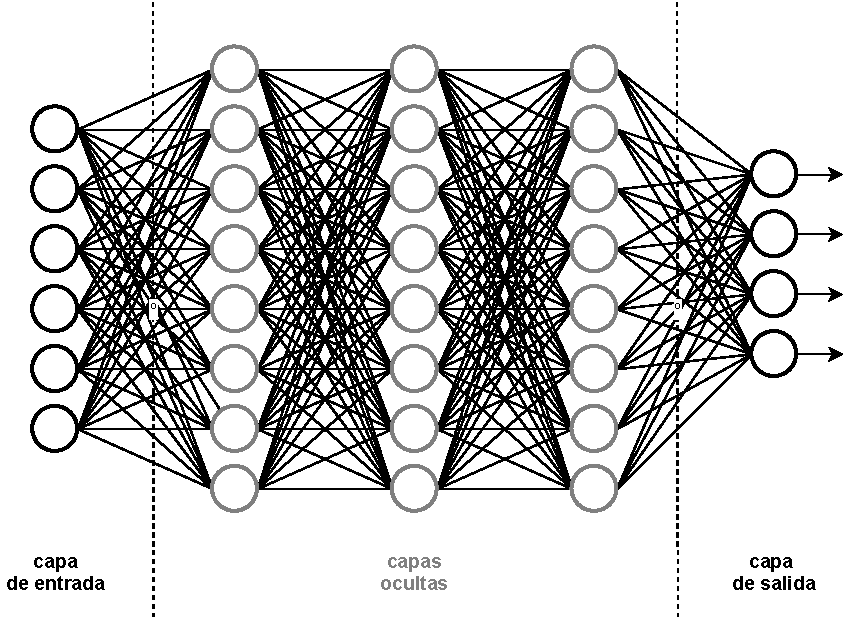
\includegraphics[width=1.1\textwidth]{figuras/desarrollo teorico/red_neuronal.pdf}
    \caption{Esquema de red neuronal artificial simple completamente conectada}
    \label{fig:red_neuronal}
\end{figure}

Como se puede ver, las neuronas se agrupan normalmente en capas de cierta profundidad, dada por el numero de neuronas en cada capa. Cada una de las capas, se interconectan totalmente entre ellas, obteniendo una topología de capas totalmente conectadas. Dentro de las capas se suele hablar de tres tipos:

\begin{itemize}
    \item \textbf{Capas de entrada}: En esta capa no existe procesamiento, ya que simplemente en estas se introducen los valores de entrada a la red. Esta tendrá tanta profundidad como datos de entrada se tengan.
    \item \textbf{Capas ocultas:} Estas capas no tienen interconexión directa con el entorno. El número de capas y su profundidad dependerán del problema que se quiera resolver.
    \item \textbf{Capas de salida:} Estas capas se corresponden con el final de nuestra red neuronal, y tendrá tanta profundidad como etiquetas o valores de salida se tengan.
\end{itemize}

\subsection{Función de Activación}

La función de transferencia comentada en el apartado anterior, se le denomina \textbf{Función de Activación}. Esta, como ya se comentó, su elección cae en función del criterio del diseñador de la red y del problema a resolver. Ahora se va a pasar a mostrar las funciones más empleadas en la actualidad.

\begin{itemize}
    \item \textbf{ReLU:} Esta función de activación sigue la expresión $a(x) = max(0,x)$. Como se puede observar se trata de una función bastante simple, ya que no requiere de ningún gran calculo, por lo que su uso está bastante extendido debido a su bajo coste computacional. Como desventaja, podemos ver que se trata de una expresión no derivable. En la figura \ref{fig:relu} se puede ver como es esta función.
    
    \begin{figure}[!ht]
    \centering
    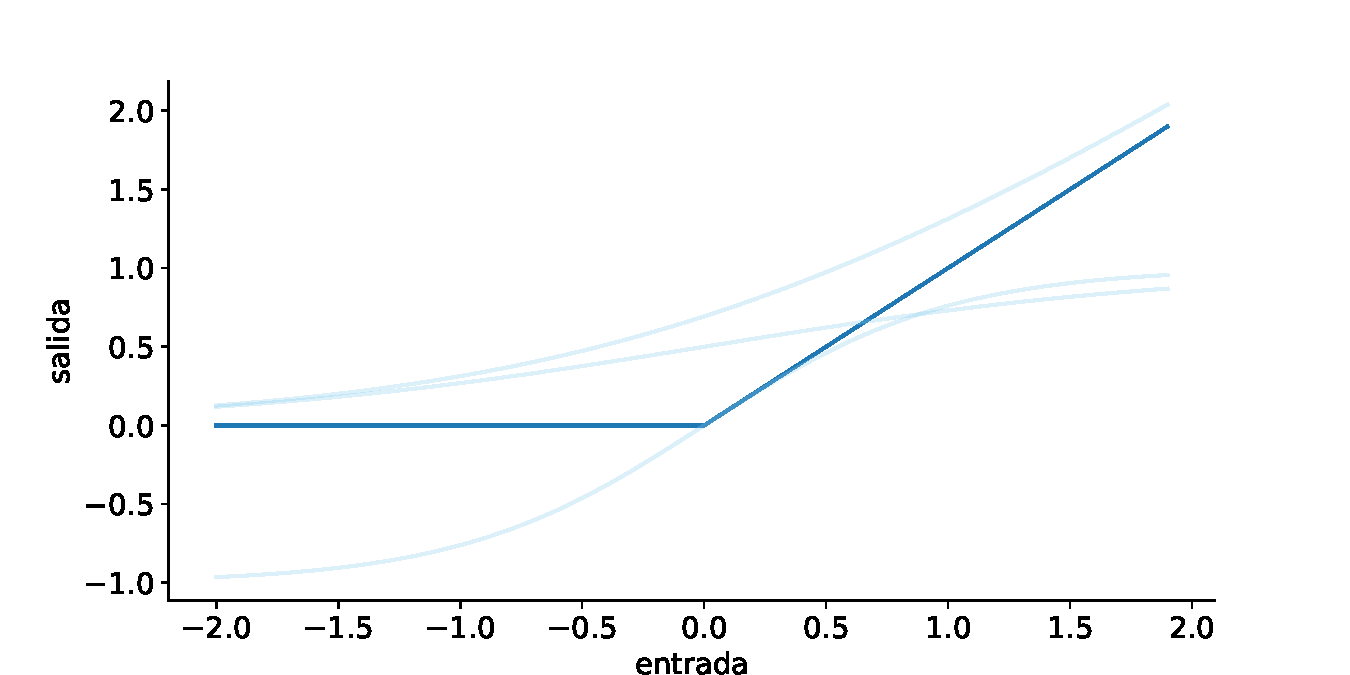
\includegraphics[width=\textwidth]{figuras/desarrollo teorico/relu.pdf}
    \caption{Representación de función de activación ReLU}
    \label{fig:relu}
    \end{figure}

    
    \item \textbf{Softplus:} Esta función de activación sigue la expresión $a(x) = log(1 + e^x)$. Como se puede observar, es una expresión bastante más compleja de resolver con respecto a la \textit{ReLU}, lo cuál se traduce en mayor coste computacional. Cómo ventaja frente a la anterior, es su derivabilidad, lo cuál lo hace adecuado para algoritmos de entrenamiento de la red que se verán posteriormente. En la figura \ref{fig:softplus} se puede ver como es esta función.
    
    \begin{figure}[!ht]
    \centering
    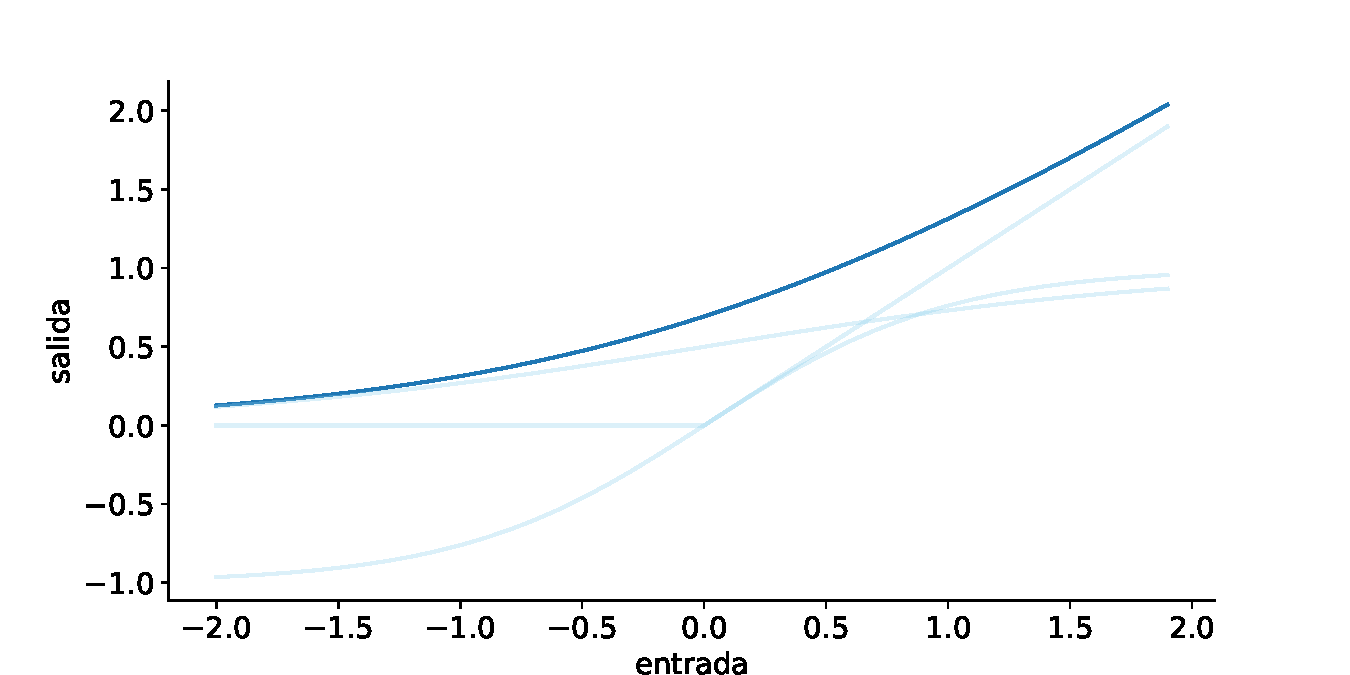
\includegraphics[width=\textwidth]{figuras/desarrollo teorico/softplus.pdf}
    \caption{Representación de función de activación Softplus}
    \label{fig:softplus}
    \end{figure}
    
    \item \textbf{Tangente hiperbólica (tanh):} Esta función de activación sigue la expresión $a(x) = tanh(x)$. Es también ampliamente usada, como la anterior, debido a su derivabilidad en todo su rango. En la figura \ref{fig:tanh} se puede ver como es esta función.
    
    \begin{figure}[!ht]
    \centering
    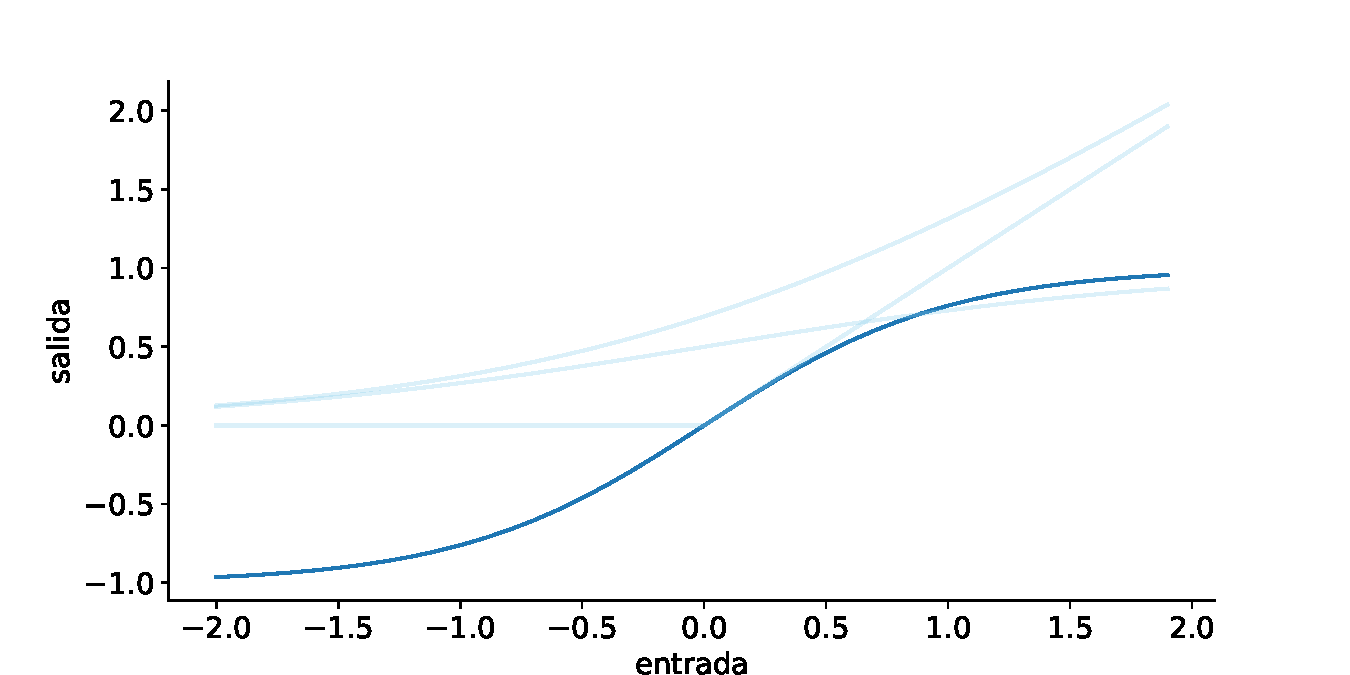
\includegraphics[width=\textwidth]{figuras/desarrollo teorico/tanh.pdf}
    \caption{Representación de función de activación tanh}
    \label{fig:tanh}
    \end{figure}
    
    \item \textbf{Sigmoide:} Esta función de activación sigue la expresión $a(x) = \frac{1}{1 + e^{-x}}$ y tiene una forma similar a la dada por la tangente hiperbólica. Comparte también que es derivable en todo su rango. En la figura \ref{fig:sigmoid} se puede ver como es esta función.
    
    \begin{figure}[!ht]
    \centering
    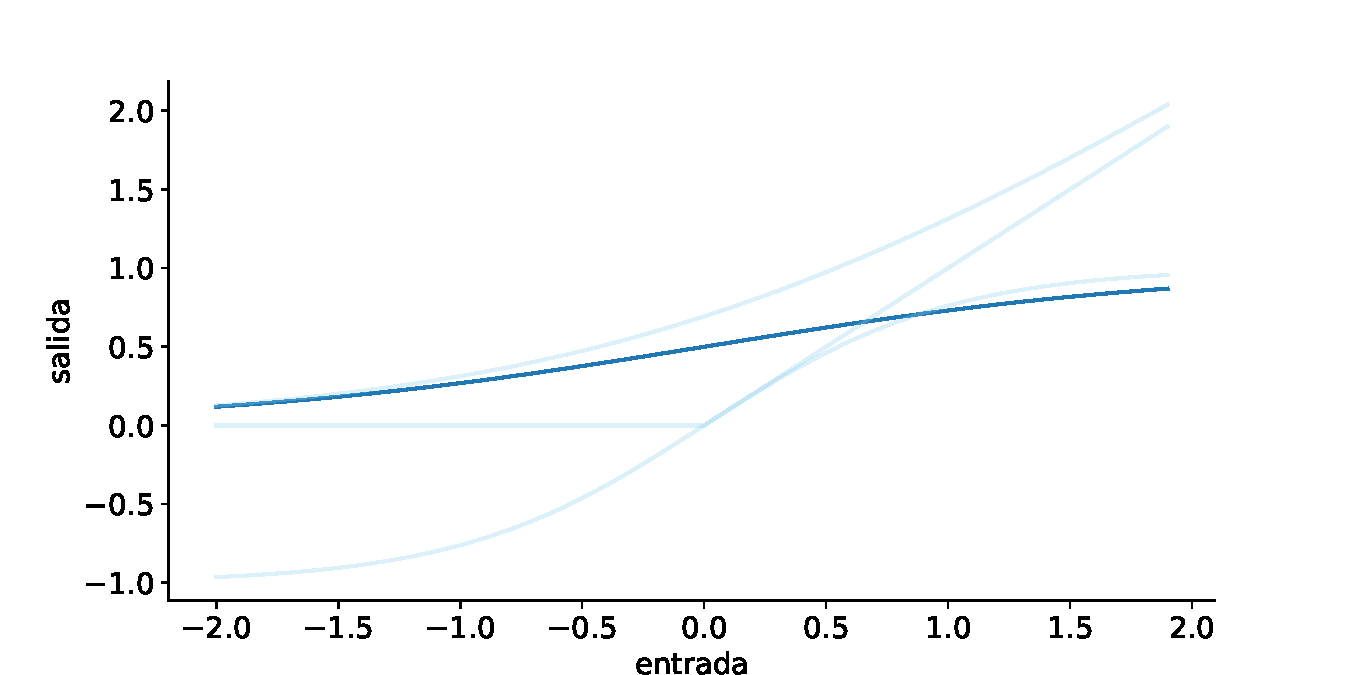
\includegraphics[width=\textwidth]{figuras/desarrollo teorico/sigmoid.pdf}
    \caption{Representación de función de activación Sigmoide}
    \label{fig:sigmoid}
    \end{figure}
    
\end{itemize}



\subsection{Entrenamiento}

Una vez diseñada como va a ser la arquitectura de la red neuronal artificial hay que comenzar a enseñarle a resolver el problema propuesto. El entrenamiento es como se conoce al proceso de aprendizaje de las redes neuronales artificiales. Este básicamente se trata de un problema de optimización de la red \cite{Aggarwal2018_training}.

Para ello se realiza una base de datos, en los cuales se conoce tanto la entrada como la salida, del problema a solucionar. De este se toma una parte, la cual irá a esta etapa de entrenamiento. El resto se empleará para la validación posterior del modelo. Normalmente se emplean más cantidad de datos para el entrenamiento que para la validación.

Los datos de entrenamiento seleccionados, se irán pasando por la red generando una salida, la cuál se comparará con la salida real y se tratará de corregir ajustando los pesos $w_i$ anteriormente comentados.

Para ver la desviación entre la salida de la red y la salida solución del problema, se emplean diferentes cálculos del error, de los que se destacan el uso de: el Error Cuadrático Medio (ECM), el Error Medio Absoluto (EAM) y la Entropía Cruzada.

La fase de optimización de este problema, trata de conseguir que el error que se acaba de comentar llegue a tener valor nulo. Las opciones de resolver este problema son bastante diferentes, pero casi todas se basan en una relación proporcional entre la variación de los pesos y el error cometido. Uno de los algoritmos más empleados para la optimización de este problema es el \textbf{Descenso del Gradiente} el cuál viene dado por la expresión \ref{eq:desc_gradiente}.

\begin{equation}
    \Delta w(t+1)= -\gamma * \nabla E(w(t))
    \label{eq:desc_gradiente}
\end{equation}

siendo $\Delta w(t+1)$ la variación de los pesos en un tiempo $t$, $\gamma$ el ratio de aprendizaje o \textit{Learning Rate} y $E$ la función de error a minimizar.

En todos los método de optimización, existe un parámetro en común, que es el \textit{Learning Rate} (LR), el cual indica el tamaño del salto en cada una de las iteraciones. Existen diferentes optimizadores que lo varían en función del resultado en las iteraciones previas.

Es totalmente vital la buena elección del valor de LR, ya que un valor muy alto de este, puede hacer que nuestro problema nunca converja, haciendo que el entrenamiento sea inútil. Por otro lado, un asignación muy bajo, hará que nuestro aprendizaje sea excesivamente lento, aunque nos asegura la convergencia. Es por ello que es primordial encontrar un valor adecuado para la resolución del problema dado.

El proceso de optimización además va acompañado de otro algoritmo necesario a la hora de deducir el error cometido por cada una de las neuronas, y así ajustar sus pesos. Es se llama \textit{Backpropagation} \cite{Goodfellow-et-al-2016} y como su nombre indica, implica el calculo del error propagándolo desde la capa de salida hasta la capa de entrada a través del resto de capas ocultas.

\subsection{\textit{Overfitting}}

Durante el aprendizaje, es necesario conseguir un numero de iteraciones adecuado para resolver nuestro problema de optimización. Esto es debido a que no es adecuado siempre que se llegue a un error de optimización igual a nulo. Esto es así, debido a que en principio, se quiere que nuestra red sea capaz de generalizar y por lo tanto, sea capaz de resolver problemas no vistos dentro del conjunto de datos de entrenamiento.

Un entrenamiento excesivo de nuestra red puede hacer que se llegue a un caso de sobre-entrenamiento o \textit{overfitting} \cite{salman2019overfitting}. Esto quiere decir que nuestra red, tan solo es capaz de resolver de forma adecuada los valores entregados en el conjunto de datos de entrenamiento, sin embargo, no es capaz de hacerlo de forma correcta con los datos de validación.

Es por ello que tras cada cierto numero de iteraciones, sea adecuado observar como resuelve la red el problema con los datos de validación, para poder establecer un punto de parada de entrenamiento de la red. Esto se ve de forma muy descriptiva en la figura \ref{fig:overfitting}.

\begin{figure}[!h]
    \centering
    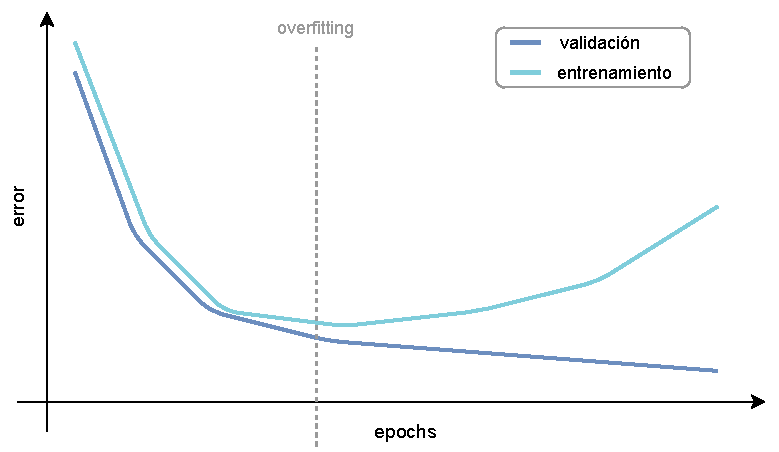
\includegraphics[width=1\textwidth]{figuras/desarrollo teorico/overfitting.pdf}
    \caption{Localización del \textit{overfitting} en un entrenamiento clásico}
    \label{fig:overfitting}
    \end{figure}

Existen diferentes tipos de entrenamiento que intentan paliar esta problemática. Estos son: el Entrenamiento estocástico y el Entrenamiento por lotes.

\begin{itemize}
    \item \textbf{Entrenamiento Estocástico} (\textit{Stochastic training}): En este tipo de entrenamiento se toman al azar de nuestro conjunto de datos, calculando su error y realizando los cambios de pesos correspondientes. Esta etapa (\textit{epoch}) habrá tantas iteraciones como datos.
    
    \item \textbf{Entrenamiento por lotes} (\textit{Batch training}): En este tipo de entrenamiento, los datos se clasifican en varios lotes aleatorios de un determinado tamaño de lote (\textit{Batch size}). En este se calcula el error a partir de la suma de los errores de cada una de las muestras de los diferentes datos. En este se consigue una mejor optimización porque se toman todos los datos de entrenamiento, pero es mas costoso cada \textit{epoch} computacionalmente hablando, ya que se necesitan muchos \textit{epochs} para la obtención de un resultado correcto.
\end{itemize}


\section{Redes Neuronales Convolucionales}

Una Red Neuronal Convolucional o \textit{Convolutional Neural Network} (CNN) es una estructura de red basada en redes neuronales. Este se encuentra dentro de la categoría de \textit{Deep Learning} debido al numero necesario de capas implicadas en este tipo de arquitecturas. Su principal diferencia con otro tipo de Redes Neuronales Artificiales es su capacidad de tomar una imagen como entrada y extraer diferentes sesgos o características de estas imágenes.

El diseño de estas redes se sigue asemejando al comportamiento de las neuronas de nuestro cerebro. En este caso inspirado en el comportamiento realizado por el córtex visual. Ambas trabajan tratando de deducir potenciales de acción de la imagen para tratar de sacar características de la misma. Esta es capaz de obtener dependencias espaciales y temporales de una imagen.

\subsection{Estructura}

Dentro de la arquitectura habitual de una CNN, existen diferentes tipos de capas esenciales que componen esta \cite{Aggarwal2018}. Cada una de ellas, se encarga de realizar unas operaciones determinadas dentro de la misma. Es por ello que para el correcto funcionamiento, es necesario conocer que actividades realiza dentro de la propia red.

En primer lugar, se debe hablar de las \textbf{Capas de Convolución}. Estas básicamente se basan en la aplicación de diferentes filtros o \textit{kernels}, que son modelados de la misma manera que son modelados los pesos dentro de una red neuronal convencional, de manera que son capaces de extraer características importantes de una imagen de entrada dada. A la salida de esta capa, encontramos los mapas de características o \textit{features maps}, los cuales son el resultado de aplicar la operación de convolución entre la imagen de entrada y el \textit{kernel}. En la figura \ref{fig:convolucion}, se puede ver un ejemplo de lo anteriormente comentado.\\

\begin{figure}[!h]
\centering
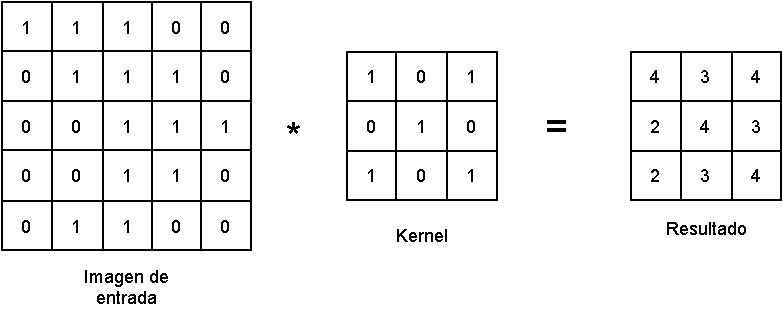
\includegraphics[width=0.9\textwidth]{figuras/desarrollo teorico/Convolucion.pdf}
\caption{Aplicación de convolución a imagen de entrada 5x5 con filtro 3x3 y \textit{stride} de 1}
\label{fig:convolucion}
\end{figure}

Las imágenes de entrada suelen tener dos dimensiones espaciales y tres canales, una por color. Es por esto que los \textit{kernel}, al aplicarse en imágenes en dos dimensiones, suelan tener de igual manera dos dimensiones. Su tamaño es variable y depende por tanto del diseñador de la arquitectura establecer un tamaño para estos, en función de las necesidades del problema a resolver. El número de \textit{kernels} que se emplean por capa también son un producto del diseñador de la arquitectura de la red y deben ser definidos al principio. A mayor cantidad de \textit{kernels}, más cantidad de características serán capaces de ser extraídas de la imagen de entrada, sin embargo, el coste computacional es mayor, sobretodo si el tamaño de los \textit{kernels} es demasiado grande, ya que supondrá en una mayor cantidad de pesos a ajustar dentro de nuestra red durante el entrenamiento.

Existe además, otro parámetro a tener en cuenta dentro de las capas convolucionales que es el \textit{stride} o paso. Este define el tamaño paso que hará el \textit{kernel} mientras recorrer la imagen para aplicar la operación de convolución. Esto es importante ya que un \textit{stride} de 2 o más conseguirá que las \textit{feature maps} de salida tengan un tamaño reducido a las de entrada.

Normalmente, junto a las capas de convolución se añaden otro dos tipos de capa: las capas de activación y las capas de \textit{batch normalization}.

\begin{itemize}
    \item \textbf{Capas de Activación:} estas siguen el mismo principio que las redes neuronales clásicas y básicamente codifica de manera que se pueda aplicar las funciones de activación de las neuronas, anteriormente vistas, a cada uno de los píxeles de la imágenes de salida o \textit{feature maps}.
    
    \item \textbf{Capas de \textit{Batch Normalization}:} estas tienen una finalidad bastante simple, y es normalizar las \textit{feature maps} de salida para que los valores que la compongan estén en un rango normalizado entre 0 y 1. 
\end{itemize}

En segundo lugar, las capas más empleadas son las \textbf{Capas de \textit{Subsampling}} o \textbf{Capas de \textit{Pooling}}. Estas capas capas se sitúan normalmente tras una capa de convolución y justamente antes de nuevamente ser convolucionada la imagen de salida. Esto es debido a que su función es reducir el tamaño de las \textit{feature maps} tratando de eliminar la información no necesaria de ella. Esto es una buena práctica debido a que reduce en gran manera el número de parámetros para siguientes capas de convolución, lo que computacionalmente es muy adecuado para la arquitectura de una red. 

Este tipo de capas no son completamente necesarias de usar, por el contrario de las capas de convolución, ya que se pueden conseguir resultados similares al aplicar \textit{stride} de valores superiores o iguales a dos en las capas de convolución. Es por ello que en algunas arquitecturas, puede ser normal no encontrarse con este tipo de capas.

Los parámetros de diseño de estas capas son el \textit{stride} que debe ser un valor superior o igual a 2, para ser capaz de reducir la dimensionalidad de las imágenes de entrada, y la función de aplicación, que no es más que filtros fijos de cierto tamaño que realizan una operación determinada al aplicar el operador de convolución. Algunas de estas son el \textit{Average Pooling}, donde se extrae el valor medio o el \textit{Max Pooling}, donde se extrae el valor más alto. En la figura \ref{fig:pooling}, podemos ver un ejemplo de aplicación de esta capa.\\

\begin{figure}[!h]
\centering
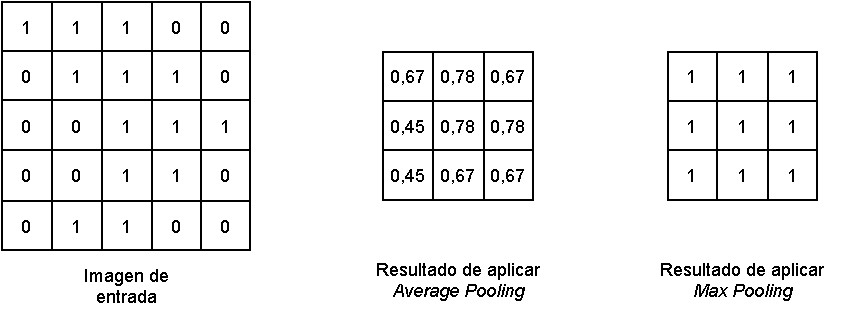
\includegraphics[width=0.95\textwidth]{figuras/desarrollo teorico/Pooling.pdf}
\caption{Aplicación de \textit{Pooling} de tamaño 3x3 a imagen de entrada 5x5 con \textit{stride} de 1}
\label{fig:pooling}
\end{figure}

Por último, para completar el proceso para la clasificación de imágenes, nos encontramos las capas de salida que son \textbf{Capas Totalmente Conectadas} o \textbf{\textit{Fuly Connected Layers}} (FL). Estas se sitúan al final de la arquitectura de la red, para convertir los \textit{feature maps} en vectores unidimensionales. Estas trabajan como una red neuronal tradicional y tienen como fin, acabar la clasificación de las imágenes de entradas en función de los valores de las características extraídas por los \textit{feature maps}.


\subsection{Arquitecturas}

Para conocer el desarrollo de las redes neuronales convolucionales, se va a tomar como referencia el desafío anual \textit{ImageNet Large Scale Visual Recognition} (ILSVRC) \cite{russakovsky2015imagenet}. En este desafío, se muestran desarrollos realizados en todo el mundo, donde diferentes arquitecturas compiten por ser la mejor y más preciso a la hora de clasificar y detectar objetos sobre la base de datos de \textit{ImageNet} \cite{5206848}. Este conjunto de datos, es uno de los más grandes existentes en la actualidad, con más de 14 millones de imágenes etiquetadas manualmente, con más de 20000 categorías diferentes. 

Algunas de las redes más importantes en los últimos años presentadas en este reto son:

\begin{itemize}
    \item \textbf{AlexNet: \cite{NIPS2012_c399862d}} Nacida en el año 2012 fue la primera vez que ganó el reto una arquitectura basad en CNN. Este año la tasa de error cometida bajó de manera considerable en comparación a años anteriores, pasando del 25\% al 17\% de error. 
    
    AlexNet era una red más compleja que las empleadas hasta el momento, y estaba compuesta por 5 capas convolucionales, 3 capas de \textit{pooling}y 3 capas \textit{fully connected} al final. Esta tenía 60 millones de parámetros y en este año se tardó en entrenar 6 días. En la figura \ref{fig:alexnet}, se puede ver una representación de como es la arquitectura de esta red.\\
    
    \begin{figure}[!h]
        \centering
        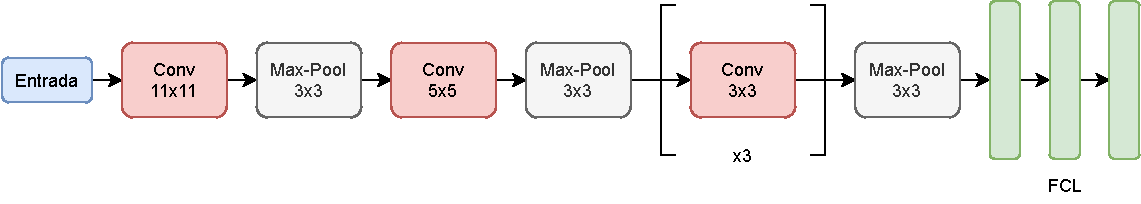
\includegraphics[width=\textwidth]{figuras/desarrollo teorico/desarrollo_teorico-AlexNet.pdf}
        \caption{Arquitectura de la red neuronal convolucional AlexNet}
        \label{fig:alexnet}
    \end{figure}
    
    En esta red, se implementa la función de activación ReLU, que hasta el momento no estaba siendo empleada. Esto aceleró de manera drástica el proceso de entrenamiento hasta en 6 veces en comparación a usar \textit{tanh} o \textit{sigmoid}, sin perder precisión.
    
    Además cabe destacar también la implementación de dos técnicas bastante novedosas para el momento: el \textit{Data Augmentation} (DA) y la técnica del \textit{Dropout} \cite{JMLR:v15:srivastava14a}. Ambas técnicas son empleadas para tratar que la red no sufra de \textit{overfitting}, pero atacando el problema desde diferentes puntos. Con el \textit{Data Augmentation}, se aumenta se añaden perturbaciones en las imágenes originales, consiguiendo una mayor cantidad de imágenes de entrenamiento. Estas perturbaciones son por ejemplo, realizar ampliaciones, rotaciones, modificar la iluminación, etc. Por otro lado, la técnica del \textit{Dropout} consiste en eliminar cierto porcentaje de neuronas de manera aleatoria de la red, haciendo que esta le cueste más aprender, y por tanto, impedir que sobreaprenda los ejemplos de los datos de entrenamiento.
    
    \item \textbf{VGGNet \cite{simonyan2015deep}:} Es el finalista del reto en 2014 y desde entonces ha sido una arquitectura ampliamente influyente. Este demostró de manera bastante intuitiva como debe ser la profundidad de una arquitectura de una red, para que trabaje de manera adecuada, ya que esto es lo que le permite extraer detalles a diferentes niveles de la imagen. Esta consiguió una tasa de error del 7,2 \%.
    
    Además, su arquitectura es bastante simple, formándose por 19 capas convolucionales con tamaños de filtro de 3x3 y \textit{stride} de 1, y capas de \textit{max pooling} con \textit{stride} de 2. En la figura \ref{fig:vggnet}, se puede ver como es la arquitectura de esta red.\\
    
    \begin{figure}[!h]
        \centering
        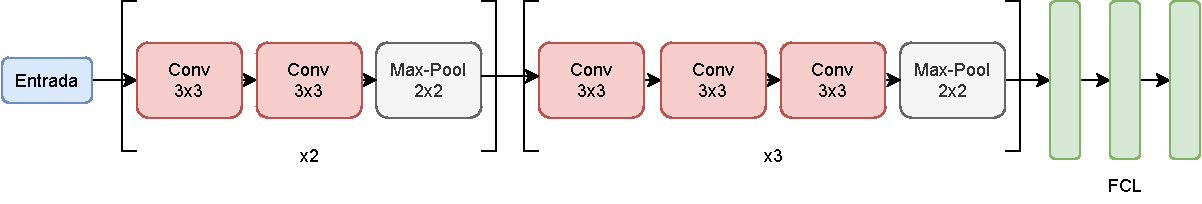
\includegraphics[width=1.05\textwidth]{figuras/desarrollo teorico/desarrollo_teorico-VGG16.pdf}
        \caption{Arquitectura de la red neuronal convolucional VGGNet}
        \label{fig:vggnet}
    \end{figure}
    
    Por otro lado, también se publicó de manera libre la configuración de los pesos que se han utilizado, por lo que sirve como base para el desarrollo de diferentes aplicaciones sin necesidad de grandes entrenamientos.
    
    \item \textbf{GoogLeNet (Inception V1): \cite{szegedy2014going}} Fue la ganadora del reto en el año 2014. Fue desarrollada por Google, pero sus autores hacen tributo a la arquitectura LeNet, en la cual se basaron en gran parte para el desarrollo de esta. Arrojó un error del 6,7 \%. Por debajo de la anteriormente comentada VGGNet.
    
    La arquitectura de esta red es bastante compleja en comparación con las existentes hasta el momento, ya que fue un modelo bastante diferente al general que había sido presentado hasta entonces. En esta se disponen varios bloques, donde se realizan diversas operaciones en paralelo, en vez de en forma secuencial como se había estado haciendo hasta este momento. En la figura \ref{fig:googlenet}, se puede ver como es la arquitectura de esta red.
    
    En esta red, se introduce por primera vez el módulo de \textbf{Inception}, que es sacado de un trabajo anterior \cite{szegedy2014going}. Un módulo Inception tiene la forma presentada en la figura \ref{fig:inception_bloque}.
    
    \begin{figure}[!h]
        \centering
        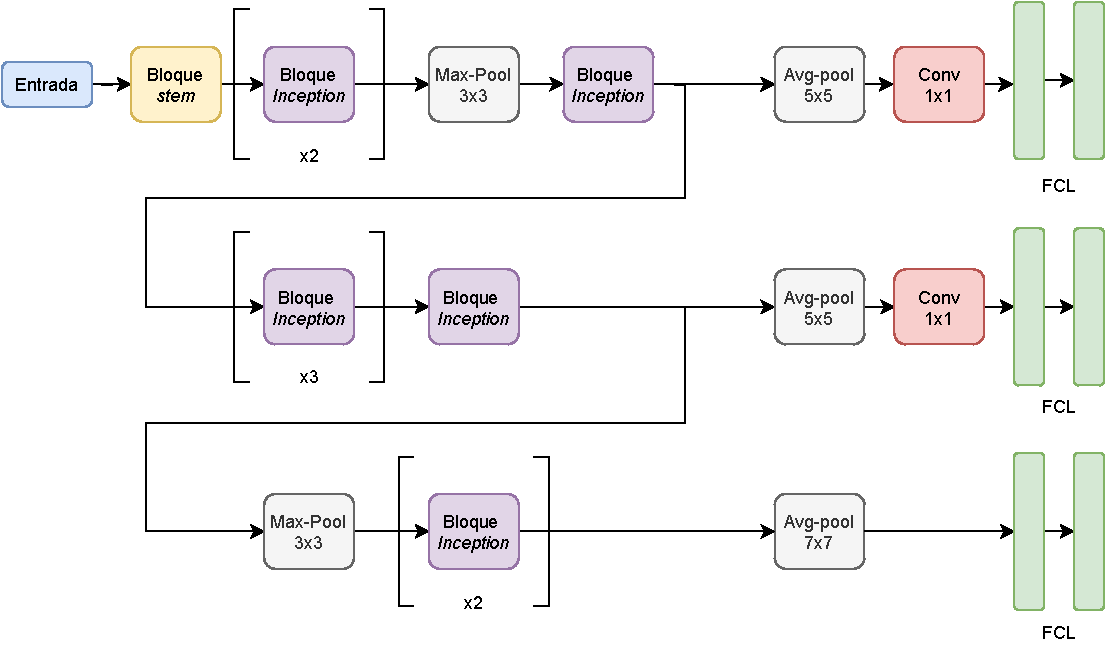
\includegraphics[width=1\textwidth]{figuras/desarrollo teorico/desarrollo_teorico-Inception V1.pdf}
        \caption{Arquitectura de la red neuronal convolucional GoogLeNet (Inception V1)}
        \label{fig:googlenet}
    \end{figure}
    
    \begin{figure}[!h]
    \centering
    \begin{subfigure}{0.45\textwidth}
        \centering
        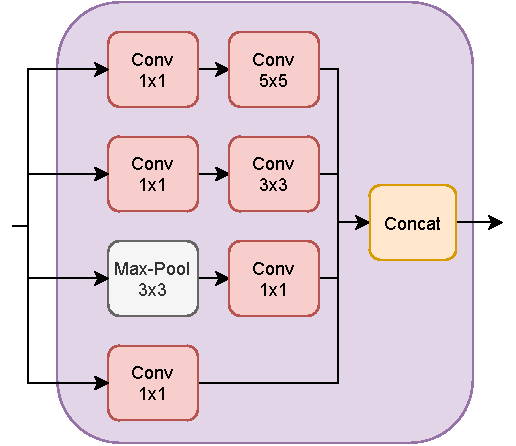
\includegraphics[width=\textwidth]{figuras/desarrollo teorico/desarrollo_teorico-Inception V1-inception.pdf} 
        \caption{Bloque \textit{Inception}}
        \label{fig:inception_bloque}
    \end{subfigure}
    \hfill\\
    \begin{subfigure}{0.65\textwidth}
        \centering
        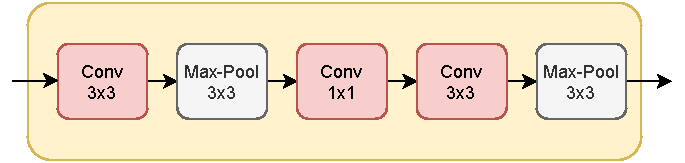
\includegraphics[width=\textwidth]{figuras/desarrollo teorico/desarrollo_teorico-Inception V1-stem.pdf} 
        \caption{Bloque \textit{stem}}
        \label{fig:stem_bloque}
    \end{subfigure}
    \caption{Bloques componentes de la arquitectura GoogleNet (Inception V1)}
    \label{fig:bloques_inceptionv1}
    \end{figure}
    
    Como se puede ver, ya no se aplica de forma secuencial la serie tradicional de capas convolucionales a la que se estaba acostumbrado, sino que el procesamiento se realiza de forma paralela, concatenando definitivamente estos procesos. Además se puede observar como realmente la aplicación de esto, no aumenta en gran medida el número de parámetros de la red y esto es debido a la aplicación de convoluciones de tamaño 1x1 que reducen de manera significativa el tamaño de la imagen de entrada. También introduce la eliminación de la capa \textit{fully connected}, sustituyéndolo por lo que llaman \textit{global average media}, que consiguiendo reducir el error en la precisión hasta en un 0,6\%.
    
    
    \item \textbf{ResNet: \cite{He2016}} Fue la ganadora del reto en el año 2015 y fue desarrollada por Microsoft. Este trabajo fue el primero en presentar redes basados en bloques residuales. Consiguió en este año bajar la tasa de error hasta un 3,57 \%, lo que marcó un gran hito en este ámbito, ya que las personas en tareas similares suelen tener una tasa de error entre el 5\% y el 10\%, dependiendo de las habilidades y experiencias de cada persona. No solo eso sino que con este concepto, se llegó a generar una red con 152 capas que era menos compleja de entrenar que la anteriormente comentada VGGNet que tan solo contaba con 19 capas de profundidad. En la figura \ref{fig:resnet}, se puede ver como es la arquitectura de esta red.
    
    \begin{figure}[!h]
        \centering
        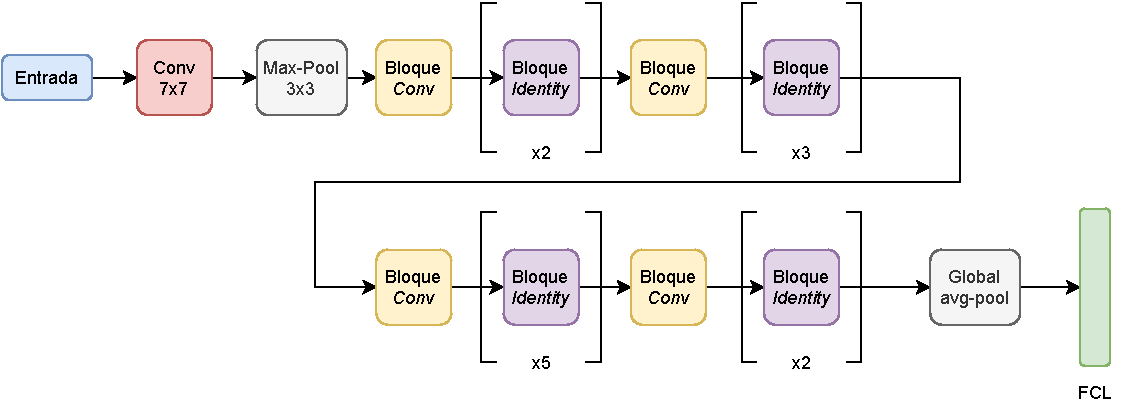
\includegraphics[width=\textwidth]{figuras/desarrollo teorico/desarrollo_teorico-ResNet 50.pdf}
        \caption{Arquitectura de la red neuronal convolucional ResNet-50}
        \label{fig:resnet}
    \end{figure}
    
    \begin{figure}[h]
    \centering
    \begin{subfigure}{0.55\textwidth}
        \centering
        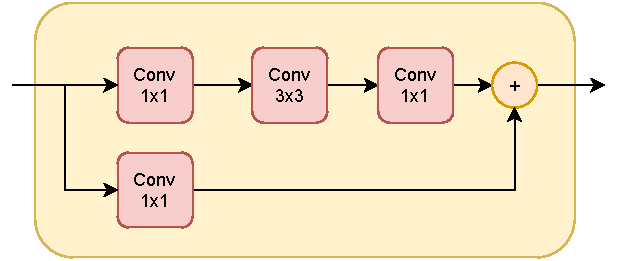
\includegraphics[width=\textwidth]{figuras/desarrollo teorico/desarrollo_teorico-ResNet 50-conv.pdf} 
        \caption{Bloque \textit{conv}}
        \label{fig:conv_bloque}
    \end{subfigure}
    \hfill
    \begin{subfigure}{0.55\textwidth}
        \centering
        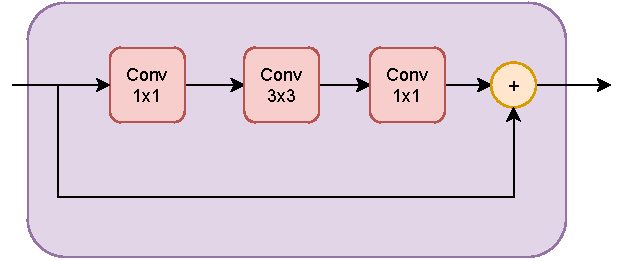
\includegraphics[width=\textwidth]{figuras/desarrollo teorico/desarrollo_teorico-ResNet 50-identity.pdf} 
        \caption{Bloque \textit{identity}}
        \label{fig:identity_bloque}
    \end{subfigure}
    \caption{Bloques componentes de la arquitectura ResNet-50}
    \label{fig:bloques_resnet50}
    \end{figure}

    
    La idea básica en la que se centra ResNet, es el tratar de dejar de apilar capas, si se esta viendo que a partir de cierto puntoesto no hace mejorar la precisión en el entrenamiento. De hecho plantean la aparición de problemas como el \textit{vanishing gradient} o el \textit{curse of dimensionality} donde la red dejaría de aprender por estos motivos.
    
    A partir de este punto nace la idea de los bloques residuales, que básicamente es una conexión que salta un cierto número de capas. En la figura \ref{fig:bloque_residual}, se puede observar como se realiza esta conexión.
    
    \begin{figure}[!h]
        \centering
        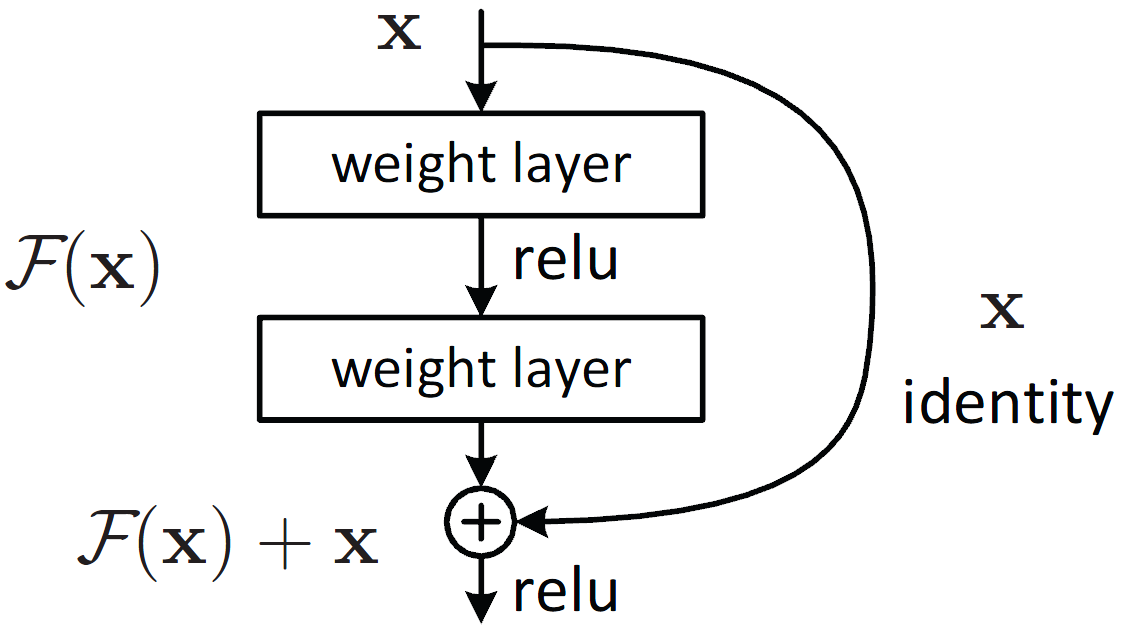
\includegraphics[width=0.5\textwidth]{figuras/desarrollo teorico/bloque_residual.png}
        \caption{Arquitectura del bloque residual \cite{He2016} propuesto para arquitecturas ResNet}
        \label{fig:bloque_residual}
    \end{figure}
    
    La idea tras estos bloques residuales, radica en introducir cierta variación en la imagen de entrada, tratando de conservar el procesado y los detalles de la imagen de entrada, junto a su contexto, que de no tener esta conexión residual, se desvanece con la profundidad de la red.
    
    
\end{itemize}